\documentclass{book}
%\usepackage{epsf}
\usepackage[dvipdfmx]{graphicx}

%\documentstyle[epsf]{jbook}
%\documentstyle[12pt,epsf]{jbook}

\title{RIKEN AICS\\
       Annual Report FY2016\\
      AICS Research Activities}
\author{}

%\setlength{\unitlength}{1cm}
%\setlength{\textwidth}{17cm}
%\setlength{\textheight}{24cm}
%\setlength{\oddsidemargin}{-1cm}
%\setlength{\evensidemargin}{-1cm}
%\setlength{\topmargin}{-0.5cm}

\begin{document}

\maketitle

\section*{Preface}

\newpage

\section*{Organization}


\tableofcontents

\part{Research Division}

\chapter{... Research Team}

\section{Members}

\begin{itemize}
  \item[] Naoya Maruyama (Team Leader)
  \item[] Motohiko Matsuda (Research Scientist)
  \item[] Shinichiro Takizawa (Research Scientist)
  \item[] Mohamed Wahib (Postdoctoral Researcher)
  \item[] Keisuke Fukuda (Research Associate)
  \item[] An Huynh (Student Trainee)
  \item[] Satoshi Matsuoka (Senior Visiting Scientist)
  \item[] Tomoko Nakashima (Assistant)
  \item[] Aya Motohashi (Assistant)
\end{itemize}


\section{Research Activities}

We develop high performance, highly productive software stacks that aim to simplify development of highly optimized, fault-tolerant computational science applications on current and future supercomputers, notably the K computer. Our current focus of work includes large-scale data processing, heterogeneous computing, and fault tolerance. A major ongoing project in our group will deliver a MapReduce runtime that is highly optimized for the intra- and inter-node architectures of the K computer as well as its peta-scale hierarchical storage systems. Another major project focuses on performance and productivity in large-scale heterogeneous systems. Below is a brief summary of each project.


\section{Research Results and Achievements}

% Matsuda & Takizawa
\subsection{KMR}

\subsubsection{A Scalable Multi-Granular Data Model for Data Parallel Workflows}

A wide range of scientific applications, including weather modeling, molecular dynamics and astrophysics, are run on large scale parallel computing systems.
Obtaining scientific insights, however, requires executing those applications multiple times typically with different parameter configurations with different applications running concurrently, composing parallel workflows.
Tasks in such a workflow typically run with multiple processes but the degree of parallelism often varies, resulting in the different numbers of tasks with the different numbers of processes.
For example, a climate simulation with data assimilation can be realized by an ensemble execution of a climate model with different input values, followed by statistical adjustment of physical properties using real observation data.
In the former phase, each task of the climate model is a parallel application with the whole simulation region split among parallel processes.
In the latter phase, a statistical analysis on each grid point in the simulation region is run using all ensemble output and observation data of the point.
Though a task in the former phase requires multiple processes, a task in the latter phase only requires a single process but the number of tasks is much larger.
Moreover, processes in each phase have completely different data access patterns.
Appropriate data decomposition and arrangement to processes are required between these two phases.
Otherwise, performance degradation occurs due to unnecessary remote access.

To efficiently execute these applications, it is necessary to satisfy requirements for degree of parallelism, number of ensembles and data access pattern of all tasks that compose the applications.
Application developers have to take the following three steps to write code that satisfies the above requirements for each task: (1) allocate enough number of processes to each ensemble, (2) decompose input data and arrange them to processes and (3) execute the task.
Coding of these steps is highly troublesome and error-prone because data arrangement in (2) requires correct decomposition and transfer of the input by considering data access pattern.
Moreover, as the implementation effort is in proportion to the number of tasks in a workflow, it becomes even worse for larger applications.
Though the above problem is a common issue for applications irrespective of science fields, there are no common effective solutions and the reality is that developers have to hand-write the troublesome codes.

To solve the problem, we propose a multi-view data model that allows the user to create multi-dimensional arrays with adaptive granularities of decomposition to achieve efficient execution of data parallel workflows.
Our framework conducts data arrangement and affinity-aware task scheduling as specified by the user with straightforward programming constructs (Fig.~\ref{takizawa_sample}).
We present a prototype implementation for distributed-memory parallel systems using MPI with APIs for C, C++, and Fortran.
A case study using a lattice QCD code called BQCD, which is developed by Nakamura from AICS Kuramashi team, demonstrates that our framework can reduce the programming effort required to implement the application compared to a conventional MPI-based implementation with performance penalties up to 17\% (Fig.~\ref{takizawa_eval_bqcd_ss,takizawa_eval_bqcd_ws}).

\begin{figure}[t]
\centering
\begin{verbatim}
   # Create a DataStore
   # Initial Split: <N,8,8,8,8>
   # Dimensions
   #   1st      : ensembles
   #   2nd - 5th: simulation space (x,y,z,t)
 1 ds0 = DataStore(4,64,64,64,64)
 2 ds0.load_parallel(task_load)

   # Execute Dirac equation solver
 3 ds0.set_split(<A,8,8,4,4>)
 4 ds0.map(ds0, task_dirac, <A,N,N,N,N>)

   # Restore to the default layout
 5 ds0.set_split(<N,8,8,8,8>)
 6 ds0.map(NULL, task_restore, <N,N,N,N,N>)
\end{verbatim}
\caption{BQCD pseudo-code that uses our model}
\label{takizawa_sample}
\end{figure}

\begin{figure}[t]
  \centering

  \subfloat[Strong Scalability] {
    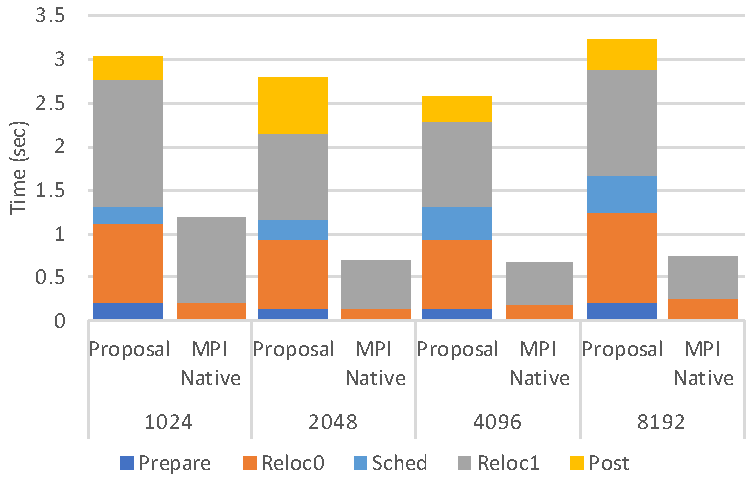
\includegraphics[width=7cm]{fig/eval_bqcd_ss.pdf}
    \label{takizawa_eval_bqcd_ss}}
  \hspace{0.1cm}
  \subfloat[Weak Scalability] {
    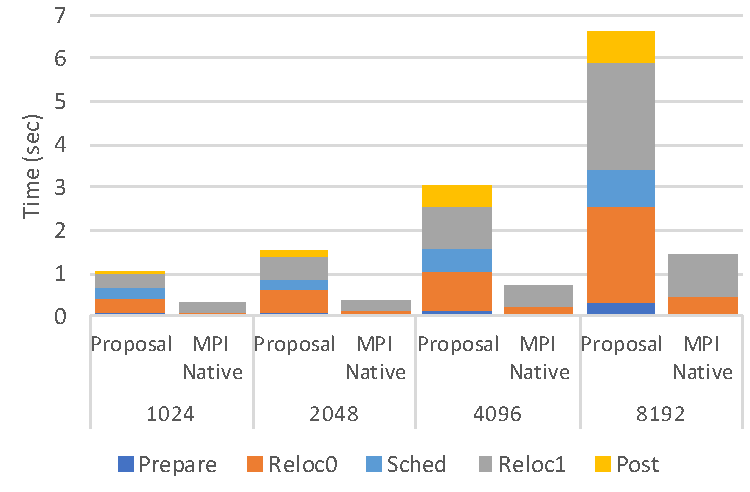
\includegraphics[width=7cm]{fig/eval_bqcd_ws.pdf}
    \label{takizawa_eval_bqcd_ws}}

  \caption{Comparison of overhead for data arrangement between our model and MPI Alltoall using BQCD}
\end{figure}



% Wahib
\subsection{High Level Framework for High Performance AMR}

% Wahib
\subsection{Extending a Global Climate Model with a High Level Framework}


\section{Schedule and Future Plan}

% Matsuda & Takizawa
\subsection{KMR}

For the scalable multi-granular data model, we plan to improve the implementation to further reduce overhead and apply it to other applications, such as weather prediction.


% Wahib
\subsection{High Level Framework for High Performance AMR}

% Wahib
\subsection{Extending a Global Climate Model with a High Level Framework}


\section{Publications}

\subsection{Journal Articles}

[1] 

[2]

[3]

\subsection{Conference Papers}

[4] Shinichiro Takizawa, Motohiko Matsuda, Naoya Maruyama, Yoshifumi Nakamura. A Scalable Multi-Granular Data Model for Data Parallel Workflows. HPC Asia 2018. 2018 (submitted).

[5]

[6]

\subsection{Posters and Presentations}

[7] Shinichiro Takizawa, Motohiko Matsuda, Naoya Maruyama. A Locality-aware Task Scheduling of Message Passing and MapReduce Hybrid Models. HPDC 2016 Poster. 2016.

[8] 滝澤 真一朗, 松田 元彦, 丸山 直也, 中村 宜文. 処理粒度に応じたデータ分割・配置を行う多次元データ処理フレームワーク. 第158回ハイパフォーマンスコンピューティング研究発表会. 2017.

[9]

\subsection{Patents and Deliverables}

[10]

[11]

[12]

\part{Operations and Computer Technologies Division}

\chapter{... Team}

\section{Members}

\section{Research Activities}

\section{Research Results and Achievements}

\subsection{Subject A...}

\subsection{Subject B...}

\section{Schedule and Future Plan}

\section{Publications}

\subsection{Journal Articles}

[1] 

[2]

[3]

\subsection{Conference Papers}

[4]

[5]

[6]

\subsection{Posters and Presentations}

[7]

[8]

[9]

\subsection{Patents and Deliverables}

[10]

[11]

[12]


\part{Flagship 2020 Project}


\chapter{Flagship 2020 Project}

\end{document}




